% % % % % % % % % % % % % % % % % % % % % % % % % % % % % % % % % % % % % % % %
% IEEE Style - Double columns, 11pt font, letterpaper
\documentclass[journal, twocolumn, final,11pt,letterpaper]{IEEEtran}	

% Include Latex Packages
\usepackage{etex}	% This package enables the use of many packages

% % Page styles
\usepackage{setspace}	% line spacing package
\doublespacing			% use double spacing
%\linespread{1.6}		% Use linespread to fine tune line spacing, not recommended


% % Figures
\usepackage{float}		% improves interface for floating objects
\usepackage{subfig}		% enables subfloat
\usepackage{graphicx}	% more image type support
\usepackage{circuitikz}
\usepackage{epstopdf}	% automatically convert included eps files to pdf
\usepackage{tikz}
%\usepackage{listings}
\usepackage{color}
\definecolor{dkgreen}{rgb}{0,0.6,0}
\definecolor{gray}{rgb}{0.5,0.5,0.5}
\definecolor{mauve}{rgb}{0.58,0,0.82}

\lstset{frame=tb,
	language=Verilog,
	aboveskip=3mm,
	belowskip=3mm,
	showstringspaces=false,
	columns=flexible,
	basicstyle={\small\ttfamily},
	numbers=none,
	numberstyle=\tiny\color{gray},
	keywordstyle=\color{blue},
	commentstyle=\color{dkgreen},
	stringstyle=\color{mauve},
	breaklines=true,
	breakatwhitespace=true,
	tabsize=3
}
\usetikzlibrary{matrix,calc}
\usetikzlibrary{shapes}

\newcommand*{\circled}[2][red]{
	\tikz[baseline=(char.base)]{
		\node[shape=ellipse,inner sep=1pt,
		draw=#1,
		] (char) {#2};}
}

%isolated term
%#1 - Optional. Space between node and grouping line. Default=0
%#2 - node
%#3 - filling color
\newcommand{\implicantsol}[3][0]{
	\draw[rounded corners=3pt, fill=#3, opacity=0.3] ($(#2.north west)+(135:#1)$) rectangle ($(#2.south east)+(-45:#1)$);
}


%internal group
%#1 - Optional. Space between node and grouping line. Default=0
%#2 - top left node
%#3 - bottom right node
%#4 - filling color
\newcommand{\implicant}[4][0]{
	\draw[rounded corners=3pt, fill=#4, opacity=0.3] ($(#2.north west)+(135:#1)$) rectangle ($(#3.south east)+(-45:#1)$);
}

%group lateral borders
%#1 - Optional. Space between node and grouping line. Default=0
%#2 - top left node
%#3 - bottom right node
%#4 - filling color
\newcommand{\implicantcostats}[4][0]{
	\draw[rounded corners=3pt, fill=#4, opacity=0.3] ($(rf.east |- #2.north)+(90:#1)$)-| ($(#2.east)+(0:#1)$) |- ($(rf.east |- #3.south)+(-90:#1)$);
	\draw[rounded corners=3pt, fill=#4, opacity=0.3] ($(cf.west |- #2.north)+(90:#1)$) -| ($(#3.west)+(180:#1)$) |- ($(cf.west |- #3.south)+(-90:#1)$);
}

%group top-bottom borders
%#1 - Optional. Space between node and grouping line. Default=0
%#2 - top left node
%#3 - bottom right node
%#4 - filling color
\newcommand{\implicantdaltbaix}[4][0]{
	\draw[rounded corners=3pt, fill=#4, opacity=0.3] ($(cf.south -| #2.west)+(180:#1)$) |- ($(#2.south)+(-90:#1)$) -| ($(cf.south -| #3.east)+(0:#1)$);
	\draw[rounded corners=3pt, fill=#4, opacity=0.3] ($(rf.north -| #2.west)+(180:#1)$) |- ($(#3.north)+(90:#1)$) -| ($(rf.north -| #3.east)+(0:#1)$);
}

%group corners
%#1 - Optional. Space between node and grouping line. Default=0
%#2 - filling color
\newcommand{\implicantcantons}[2][0]{
	\draw[rounded corners=3pt, opacity=.3] ($(rf.east |- 0.south)+(-90:#1)$) -| ($(0.east |- cf.south)+(0:#1)$);
	\draw[rounded corners=3pt, opacity=.3] ($(rf.east |- 8.north)+(90:#1)$) -| ($(8.east |- rf.north)+(0:#1)$);
	\draw[rounded corners=3pt, opacity=.3] ($(cf.west |- 2.south)+(-90:#1)$) -| ($(2.west |- cf.south)+(180:#1)$);
	\draw[rounded corners=3pt, opacity=.3] ($(cf.west |- 10.north)+(90:#1)$) -| ($(10.west |- rf.north)+(180:#1)$);
	\fill[rounded corners=3pt, fill=#2, opacity=.3] ($(rf.east |- 0.south)+(-90:#1)$) -|  ($(0.east |- cf.south)+(0:#1)$) [sharp corners] ($(rf.east |- 0.south)+(-90:#1)$) |-  ($(0.east |- cf.south)+(0:#1)$) ;
	\fill[rounded corners=3pt, fill=#2, opacity=.3] ($(rf.east |- 8.north)+(90:#1)$) -| ($(8.east |- rf.north)+(0:#1)$) [sharp corners] ($(rf.east |- 8.north)+(90:#1)$) |- ($(8.east |- rf.north)+(0:#1)$) ;
	\fill[rounded corners=3pt, fill=#2, opacity=.3] ($(cf.west |- 2.south)+(-90:#1)$) -| ($(2.west |- cf.south)+(180:#1)$) [sharp corners]($(cf.west |- 2.south)+(-90:#1)$) |- ($(2.west |- cf.south)+(180:#1)$) ;
	\fill[rounded corners=3pt, fill=#2, opacity=.3] ($(cf.west |- 10.north)+(90:#1)$) -| ($(10.west |- rf.north)+(180:#1)$) [sharp corners] ($(cf.west |- 10.north)+(90:#1)$) |- ($(10.west |- rf.north)+(180:#1)$) ;
}

%Empty Karnaugh map 4x4
\newenvironment{Karnaugh}%
{
	\begin{tikzpicture}[baseline=(current bounding box.north),scale=0.8]
	\draw (0,0) grid (4,4);
	\draw (0,4) -- node [pos=0.9,above right,anchor=south west] {C1C0} node [pos=0.9,below left,anchor=north east] {EQ} ++(135:1);
	%
	\matrix (mapa) [matrix of nodes,
	column sep={0.8cm,between origins},
	row sep={0.8cm,between origins},
	every node/.style={minimum size=0.3mm},
	anchor=8.center,
	ampersand replacement=\&] at (0.5,0.5)
	{
		\& |(c00)| 00         \& |(c01)| 01         \& |(c11)| 11         \& |(c10)| 10         \& |(cf)| \phantom{00} \\
		|(r00)| 00             \& |(0)|  \phantom{0} \& |(1)|  \phantom{0} \& |(3)|  \phantom{0} \& |(2)|  \phantom{0} \&                     \\
		|(r01)| 01             \& |(4)|  \phantom{0} \& |(5)|  \phantom{0} \& |(7)|  \phantom{0} \& |(6)|  \phantom{0} \&                     \\
		|(r11)| 11             \& |(12)| \phantom{0} \& |(13)| \phantom{0} \& |(15)| \phantom{0} \& |(14)| \phantom{0} \&                     \\
		|(r10)| 10             \& |(8)|  \phantom{0} \& |(9)|  \phantom{0} \& |(11)| \phantom{0} \& |(10)| \phantom{0} \&                     \\
		|(rf) | \phantom{00}   \&                    \&                    \&                    \&                    \&                     \\
	};
}%
{
	\end{tikzpicture}
}

%Empty Karnaugh map 2x4
\newenvironment{Karnaughvuit}%
{
	\begin{tikzpicture}[baseline=(current bounding box.north),scale=0.8]
	\draw (0,0) grid (4,2);
	\draw (0,2) -- node [pos=0.7,above right,anchor=south west] {LA/LB} node [pos=0.6,below left,anchor=north east] {S} ++(120:1);
	%
	\matrix (mapa) [matrix of nodes,
	column sep={0.8cm,between origins},
	row sep={0.8cm,between origins},
	every node/.style={minimum size=0.3mm},
	anchor=4.center,
	ampersand replacement=\&] at (0.5,0.5)
	{
		\& |(c00)| 00         \& |(c01)| 01         \& |(c11)| 11         \& |(c10)| 10         \& |(cf)| \phantom{00} \\
		|(r00)| 0             \& |(0)|  \phantom{0} \& |(1)|  \phantom{0} \& |(3)|  \phantom{0} \& |(2)|  \phantom{0} \&                     \\
		|(r01)| 1             \& |(4)|  \phantom{0} \& |(5)|  \phantom{0} \& |(7)|  \phantom{0} \& |(6)|  \phantom{0} \&                     \\
		|(rf) | \phantom{00}  \&                    \&                    \&                    \&                    \&                     \\
	};
}%
{
	\end{tikzpicture}
}

%Empty Karnaugh map 2x2
\newenvironment{Karnaughquatre}%
{
	\begin{tikzpicture}[baseline=(current bounding box.north),scale=0.8]
	\draw (0,0) grid (2,2);
	\draw (0,2) -- node [pos=0.7,above right,anchor=south west] {b} node [pos=0.7,below left,anchor=north east] {a} ++(135:1);
	%
	\matrix (mapa) [matrix of nodes,
	column sep={0.8cm,between origins},
	row sep={0.8cm,between origins},
	every node/.style={minimum size=0.3mm},
	anchor=2.center,
	ampersand replacement=\&] at (0.5,0.5)
	{
		\& |(c00)| 0          \& |(c01)| 1  \\
		|(r00)| 0 \& |(0)|  \phantom{0} \& |(1)|  \phantom{0} \\
		|(r01)| 1 \& |(2)|  \phantom{0} \& |(3)|  \phantom{0} \\
	};
}%
{
	\end{tikzpicture}
}

%Defines 8 or 16 values (0,1,X)
\newcommand{\contingut}[1]{%
	\foreach \x [count=\xi from 0]  in {#1}
	\path (\xi) node {\x};
}

%Places 1 in listed positions
\newcommand{\minterms}[1]{%
	\foreach \x in {#1}
	\path (\x) node {1};
}

%Places 0 in listed positions
\newcommand{\maxterms}[1]{%
	\foreach \x in {#1}
	\path (\x) node {0};
}

%Places X in listed positions
\newcommand{\indeterminats}[1]{%
	\foreach \x in {#1}
	\path (\x) node {X};
}



% % Maths
\usepackage[cmex10]{amsmath}	% Maths
\usepackage{amsfonts,amssymb} 	% maths symbols

% % Tables
\usepackage{booktabs}  % professional-looking tables
\usepackage{multicol} %used for getting multicolumn without page-break
\usepackage{multirow}	% multi-row tables
\usepackage{array}		% define column format of a table

% % Others
\usepackage{caption}	%Customising captions in floating environments
%\usepackage{abstract}
\usepackage{cite}		% cite multiple
\usepackage{fixltx2e}	%added by pilawa, preventing figure* to get ahead of regular figures.
\usepackage{url}		% url display

% %
\hyphenation{op-tical net-works semi-conduc-tor}	% correct bad hyphenation here
\providecommand{\e}[1]{\ensuremath{\times 10^{#1}}}		% use use \e{2} for scientific number expression


% % Optional packages that might be useful
%\usepackage{epsf}		% eps fix
%\usepackage{verbatim}	% verbatim text are not interpreted by the compiler 
%\numberwithin{equation}{section}	% number equation according to section
%\usepackage{xfrac}		% slanted fraction
%\usepackage{pgfplots}	% plot graph
%\usepackage{tikz,pgfplots} % plot graph
%\usepackage{endnotes}	% endnotes


% Title of Document
\title{ECE385 Experiment \#3
	}
\author{
\IEEEauthorblockN{Eric Meyers, Ryan Helsdingen}\\
\IEEEauthorblockA{Section ABG; TAs: Ben Delay, Shuo Liu \\
February 10th, 2016 \\
emeyer7, helsdin2}}
% % % % % % % % % % % % % % % % % % % % % % % % % % % % % % % % % % % % % % % 
\begin{document}
	
%SECTION : Formatting and Title
\maketitle
\singlespacing

%SECTION 1 - Introduction - Eric
\section{Introduction}
\IEEEPARstart{T}{he} purpose of this lab is to design and construct a four-bit serial logic processor that performs a total of eight logical operations in a bit-wise fashion. There are two four-bit words stored in two shift registers. WRITE MORE SHIT HERE \\
\vspace{-5mm}

%SECTION 2 - Pre-Lab  - Eric
\section{Pre-Lab}
Part A) Describe the simplest (two-input one-output) circuit that can optionally invert a signal (i.e., one input determines if the output is equal to the other input or equal to the other input inverted). Sketch your circuit. \\

Answer: The logic needed is shown in the following truth table:
\begin{center}
	\begin{tabular}{ll|l}
		A & B & Y \\ \hline
		0 & 0 & 0 \\
		0 & 1 & 1 \\
		1 & 0 & 1 \\
		1 & 1 & 0 \\
	\end{tabular}
\end{center}

Taking B to be the "select" line in this example, when the input (A) is driven high and our select line (B) is low, the output will be high. The reverse case is true when the input (A) is low and the select line (B) is high, the output will also be high. Therefore, depending on the select line, the input will be inverted. This can be implemented with a single XOR gate as shown below. \\
\begin{center}
	\begin{circuitikz} \draw
	(2,1) node[xor port] (myxor) {}
	(myxor.in 1) node[left=.5cm](a) {A}
	(myxor.in 2) node[left = .5cm](b) {B}
	(myxor.out)node[right = .5cm](y){Y};
	\end{circuitikz}
\end{center}
\vspace{5mm}

Part B) Explain how a modular design such as that presented above improves testability and cuts down development time. Propose an approach that could be used to troubleshoot the modular circuit above if it appeared to be completing the computation cycle correctly but was not giving the correct output. (Be specific.)\\

Answer: A modular design allows the operator to unit-test each individual module. Once each module is successfully tested, the entire system can be integrated into a whole-system and tested. A modular design ideally will cut down the debugging time needed on the system as a whole.  


%SECTION 3 - Description of Circuit - Eric
\section{Description of Circuit}
The logic processor was designed to contain two storage registers, and allow the operator to specify the data loaded into each register (A and B), as well as the operation performed between the two register, where the output is stored and 
The team designed a total of four modular sub-systems in this lab. The following sub-systems were designed and constructed:\\
\begin{enumerate}
	\item Data Loader Unit
	\item Computation Unit
	\item Function-Select and Output Router Unit
	\item Control Logic Finite State Machine (FSM) Unit
\end{enumerate}
\vspace{2mm}

Each sub-system was tested individually and system integration tests were performed at the end upon successfully unit-testing each component. This way the team could eliminate errors and debug with efficiency.\\

A total of eight operations can be performed on this unit. AND, OR, XOR, NAND, NOR, and NXOR are the six primary logical operations that can be performed, along with the last two operations simply being loading the specified registers with all 1s or 0s. \\

The Data Loader consists of a total of six switches. Two switches for loading either register A or B, and four switches to specify the contents to store in the particular register.\\

The Computation Unit performed the selected operation specified through the three function-select switches. The output of the operation is funnelled into the proper register as given by the operator. \\

Finally, the Control Logic/Finite State Machine Unit is a sequential circuit that essentially determines the correct  number of cycles to perform a full logical operation. It relies on one input (execute switch) and has one output that determines if the registers should be shifting right, doing nothing, or loading. \\

In the end, the functionality of the circuit is as follows: when a user selects a four-bit word and loads it into the register of their choosing, they must then select the logical operation they would like to perform, select where they would like the output of this logical operation to go via the routing selection, and flip the execute switch. This will begin shifting the outputs of the shift register and perform bitwise logical operations of the requestion function. The machine will halt after exactly four operations and the register requested through the routing switches will contain the output of the logical operation. \\

%SECTION 4 - State Diagram - Eric
\section{State Diagram}
The FSM created in this lab is a Mealy State Machine and this was chosen due to the simplicity of the relationship between the input and output on the state diagram.

\begin{figure} [H]
	\centering
	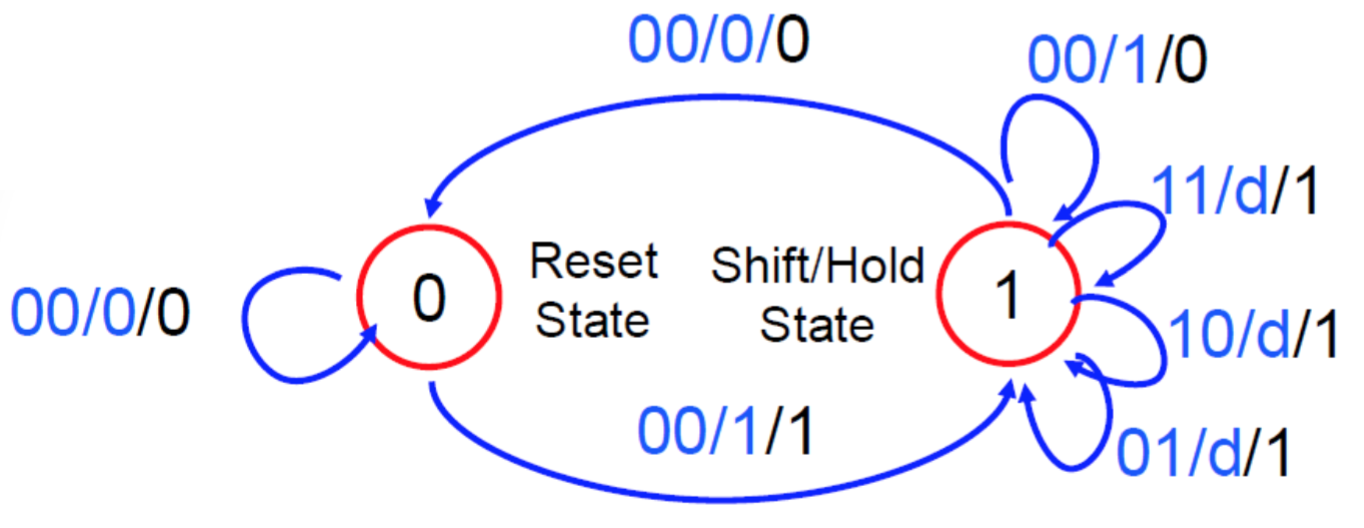
\includegraphics[scale=0.35]{FSM.png}
	\label{fig:mealy-fsm}
	\caption{Mealy FSM}
\end{figure}    

%SECTION 5 - Design - Eric
\section{Design}
The first component designed in this lab was the FSM Sequential Logic Circuit. This is because the output of this state machine controls the actions on the shift register (i.e. this output controls the "control bits", S1 and S0, which determines whether the registers are shifting right, parallel loading, or doing nothing). This is important because it determines whether we are in a load/execute/do nothing state. \\

The truth table was given from the documentation in the Experiment 3 PDF. This is shown below in figure:.

\begin{figure} [H]
	\centering
	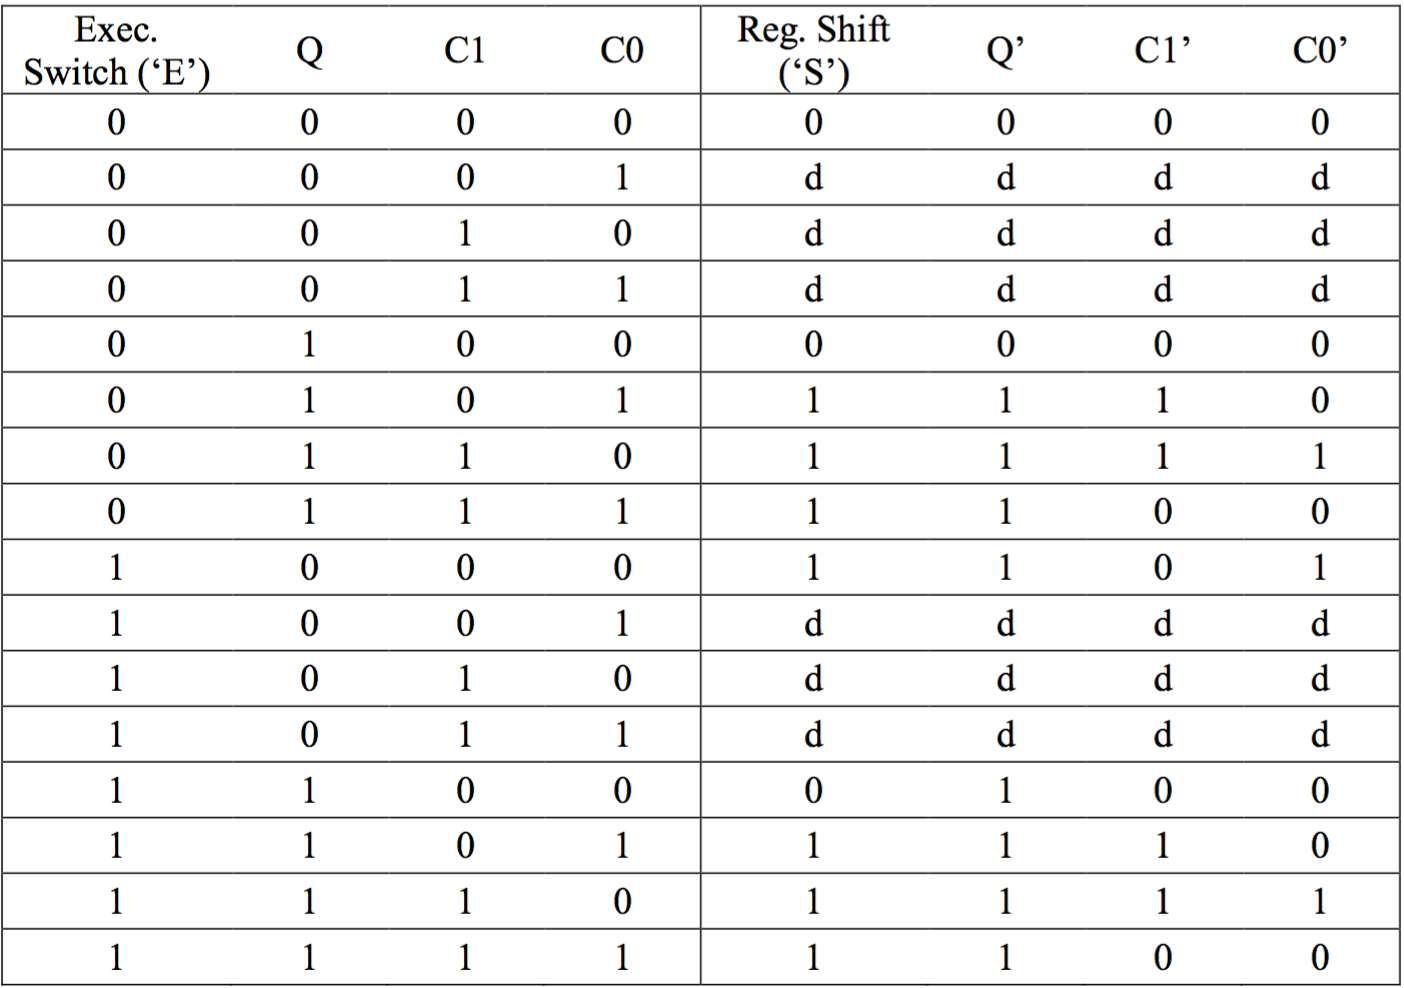
\includegraphics[scale=0.33]{FSM_Truth_Table.png}
	\label{fig:fsm-truth-table}
	\caption{FSM Truth Table}
\end{figure}       

Next, given this truth table, the team constructed a K-Map for each of the output bits - S, Q , C1 and C0. Since the only output is "S" and the remaining bits are only internal to the state machine, the 


The first component that was designed was the Loader Unit. As stated before, this requires the operator to input the four bits of data via the DIN switches, and allows them to either load it into the A register or the B register. If either LoadA or LoadB are on, the  Only when LoadA OR LoadB is on, must the contents specified by DIN have the ability to be parallel loaded into the shift register. \\

Next, the FSM Sequential Logic Circuit was designed 



\begin{figure} [H]
	\centering
	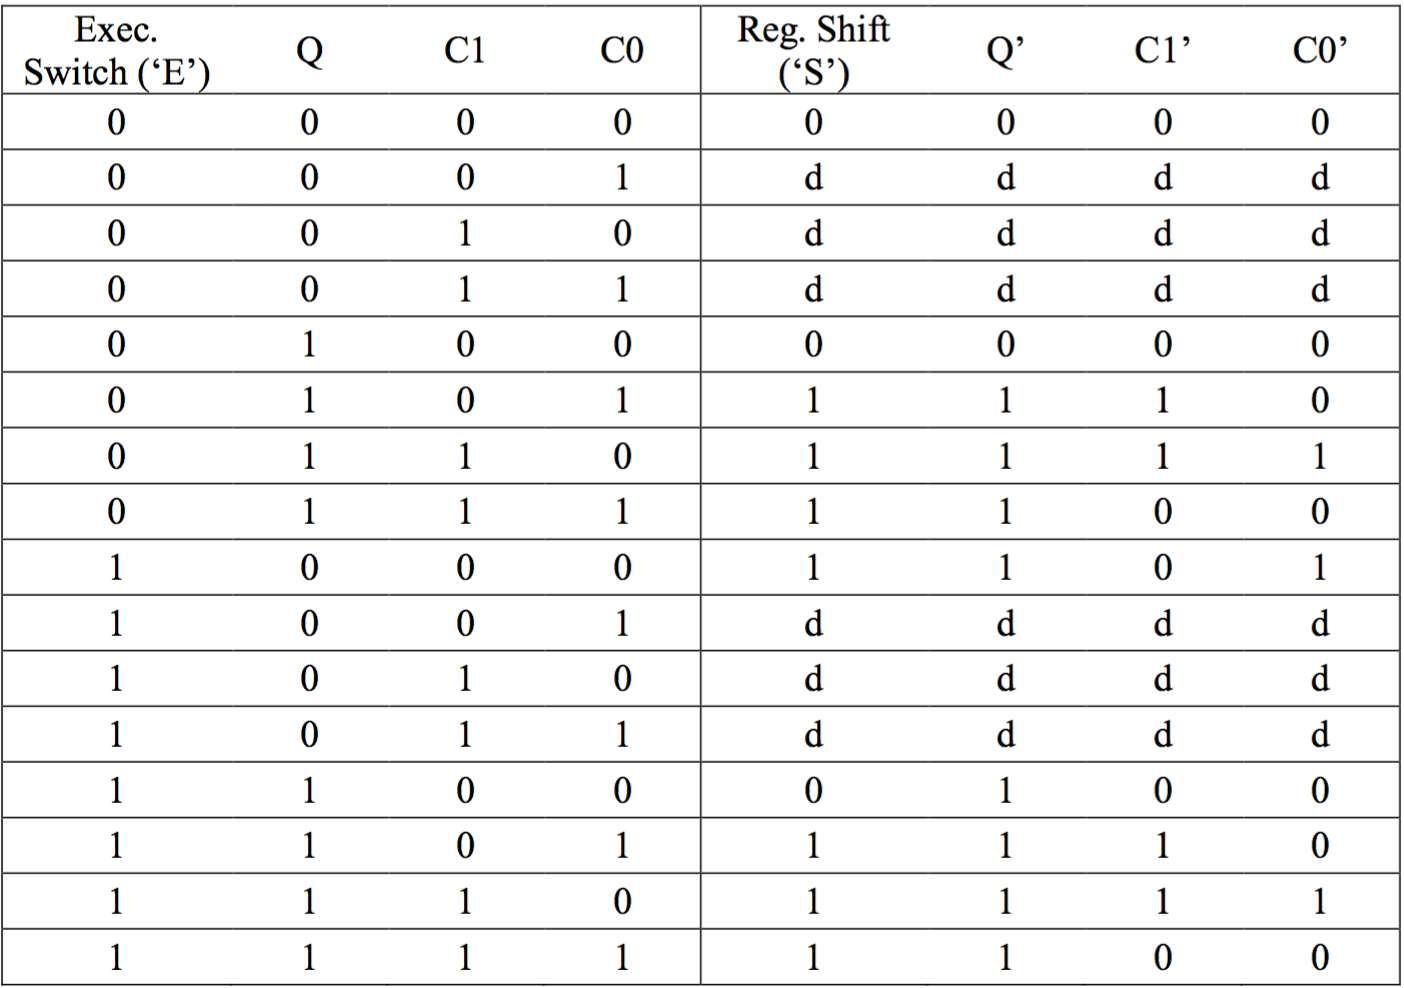
\includegraphics[scale=0.33]{FSM_Truth_Table.png}
	\label{fig:fsm-truth-table}
	\caption{FSM Truth Table}
\end{figure}            

\begin{center}
	\begin{tabular}{lll|ll|ll}
		S & LA & LB & S1A & S0A & S1B & S0B\\ \hline
		0 & 0 & 0 & 0 & 0 & 0 & 0 \\
		0 & 0 & 1 & 0 & 0 & 1 & 1 \\
		0 & 1 & 0 & 1 & 1 & 0 & 0 \\
		0 & 1 & 1 & 1 & 1 & 1 & 1 \\
		1 & 0 & 0 & 0 & 1 & 0 & 1 \\
		1 & 0 & 1 & 0 & 0 & 1 & 1 \\
		1 & 1 & 0 & 1 & 1 & 0 & 0 \\
		1 & 1 & 1 & 1 & 1 & 1 & 1 \\
	\end{tabular}
\end{center}
%SECTION 6 - Block Diagram - Ryan
\section{Block Diagram} 
Please refer to Figure \_\_\_\_ in "Section XI: Figures" of this document to view the Block Diagram created in this lab.
 
%SECTION 7 - Circuit/Logic Diagrams - Eric
\section{Circuit/Logic Diagrams}
As stated before, to allow for easier  construction and debugging, this system was broken down into modular components. All circuit diagrams are shown in "Section XI: Figures" of this document.\\
 
The FSM Control Logic is shown in Figure \_\_\_. The Loader/Computation/Router Unit are shown in Figure \_\_\_.
 
%SECTION 8 - Component Layout Sheet - Eric 
\section{Component Layout Sheet}
Please refer to Figure \_\_\_\_ in "Section XI: Figures" of this document to view the Component Layout Sheet created in this lab.

%SECTION 9 - Documentation - Ryan
\section{Documentation from Experiment}
RYAN SECTION


%SECTION 10 - Conclusion - Ryan
\section{Conclusion}
RYAN SECTION

\newpage
\onecolumn
%SECTION 11: Figures
\section{Figures}


%SECTION : Bibliography
%Insert Bibliography if needed

\end{document}